% Ch5.tex

\chapter{Frog call classification based on multi-label learning}
\label{cha:cha7ML}
\textbf{Research problem}
\\
In Chapter \ref{cha:cha6MIML}, the classification performance is highly affected by the syllable segmentation results, which is realised by acoustic event detection (AED). 
\\
\textbf{Research sub-question}
\\
How to reduce the effect of AED results and classify multiple simultaneously vocalising frog species in low SNR recordings?


\section{Overview}
\label{sect:introduction}

This chapter describes the research conducted for classifying multiple simultaneously vocalising frog species. In Chapter \ref{cha:cha6MIML}, acoustic features are calculated based on acoustic event detection (AED) results, but the multiple-instance multiple-label (MIML) classification performance is highly affected by the accuracy of AED results. To reduce the bias introduced by AED, this chapter uses global feature sets for classifying multiple frog species in field recordings.
To be specific, three features are calculated: linear prediction coefficients (LPCs), Mel-frequency cepstral coefficients (MFCCs), and adaptive-frequency scaled wavelet packet decomposition sub-band cepstral coefficients (AWSCCs). Here, each feature is extracted from the whole 10-second recording without syllable segmentation. Two cepstral feature sets are constructed by statistical analysis and spectral clustering. Since each 10-second recording is represented by a whole feature set and has multiple frog species, the classification process can be naturally framed as a multiple-label (ML) learning framework.  


\section{Methods}

\subsection{Acquisition of frog call recordings}

To evaluate the proposed algorithm, the same dataset with Chapter~\ref{cha:cha6MIML} is used. The description of this dataset can be found in Chapter~\ref{chap5:Materials}. We first manually inspect spectrograms of ten randomly selected call examples for each frog species. Dominant frequency of each frog species as listed in Table~\ref{tab:JCU} is used as prior information for subsequent analysis.



\subsection{Feature extraction}
Extracting discriminating features, which maximise between-group (inter-specie) dissimilarity and minimise within-group (intra-specie) dissimilarity, is very important for achieving high classification performance \citep{huang2009frog, bedoya2014automatic}. In this chapter, three global features are calculated to classify multiple simultaneously vocalising frog species in each 10-second recording: LPCs, MFCCs, and AWSCCs. 


\textit{LPCs}: Linear prediction coding (LPCs) is often used to represent the spectral envelope of speech sounds \citep{itakura1975line}. LPCs coefficients can be calculated using a linear predictive filter.

\begin{equation}
X(n) = \sum_{i}^{p}a_{i}x(n-i)
\end{equation}
where $p$ is the order of the polynomial $a_{i}$. In the proposed study, the value of $p$ is set at 12 (12th-order polynomial), and 13 LPCs coefficients are calculated. For those frog vocalizations with different spectral envelopes, LPCs can obtain a high classification accuracy, and has been widely used in previous studies \cite{yuan2013frog, jaafarcomparative, jaafar2015effect}.

\textit{MFCC}: The description for calculating MFCCs can be found in Chapter~\ref{cha:cha4EnhancedFeature}. 


\textit{AWSCCs}: To calculate AWSCCs, constructing a suitable frequency scale for a WP tree based on the dominant frequency of each frog species is the first step, because different frog species tend to have different dominant frequencies \citep{Gingras2013}. In Chapter \ref{cha:cha5WaveletFeature}, k-means clustering was first applied to the extracted dominant frequencies of training data. Then, the frequency scale was built by sorting clustering centroids to construct the WP tree. In this chapter, the prior information for dominant frequency ($F_{0}$) (see Table~\ref{tab:JCU}) is directly used to construct the WP tree. Then, the steps for calculating AWSCCs are the same with Chapter~\ref{cha:cha5WaveletFeature}. 

\subsection{Feature construction}

Cepstral features are calculated of each frame, where each windowed signal contains $n$ 12-dimensional feature vectors. Then, two methods are used to compute a reduced set of features. 

The first method is to compute six statistical values for representing $n$ 12-dimensional MFCCs \citep{dufour2013clusterized}. Let MFCCs of each windowed signal be $V_{i}{i=1,...,12}$, $d$ and $D$ are used to represent the velocity and acceleration of $V$.


then the six statistical values are calculated as follows:

\begin{equation}
f_{1} = \frac{\sum_{i=1}^{n}V_{i}}{n}
\end{equation}

 
 \begin{equation}
 f_{2} = \sqrt{\frac{1}{n-1}\sum_{i=1}^{n}(V_{i}-f_{1})^{2}}
 \end{equation}


\begin{equation}
f_{3} = \sqrt{\frac{1}{n-2}\sum_{i=1}^{n}(d-d_{i}^{2}}
\end{equation}


\begin{equation}
f_{4} = \sqrt{\frac{1}{n-3}\sum_{i=1}^{n}(D-D_{i})^{2}}
\end{equation}



\begin{equation}
f_{5} = \frac{\sum_{i=1}^{n-1}|d_{i}|}{n-1}
\end{equation}


\begin{equation}
f_{6} = \frac{\sum_{i=1}^{n-2}D_{i}}{n-2}
\end{equation}


Finally, each windowed signal is represented as the concatenation of the six above features for the 12 cepstral coefficients, where the dimension of our feature set is 72.


The second method first clusters the 12 cepstral coefficients of all the windowed signal. Here, k-means clustering is used to reduce the preliminary dimension of all 12 cepstral coefficients. 
Then, dynamic time warping is used to calculate the distance between each clustered cepstral coefficients. Finally, spectral clustering is applied for further dimension reduction and getting the final feature vector. In this chapter, the value of $k$ for k-means clustering is 50, and the number of clusters for spectral clustering is experimentally set at 2. Finally, the dimension of our constructed feature set is 24.


\begin{figure}[htb!] % Example image
\center{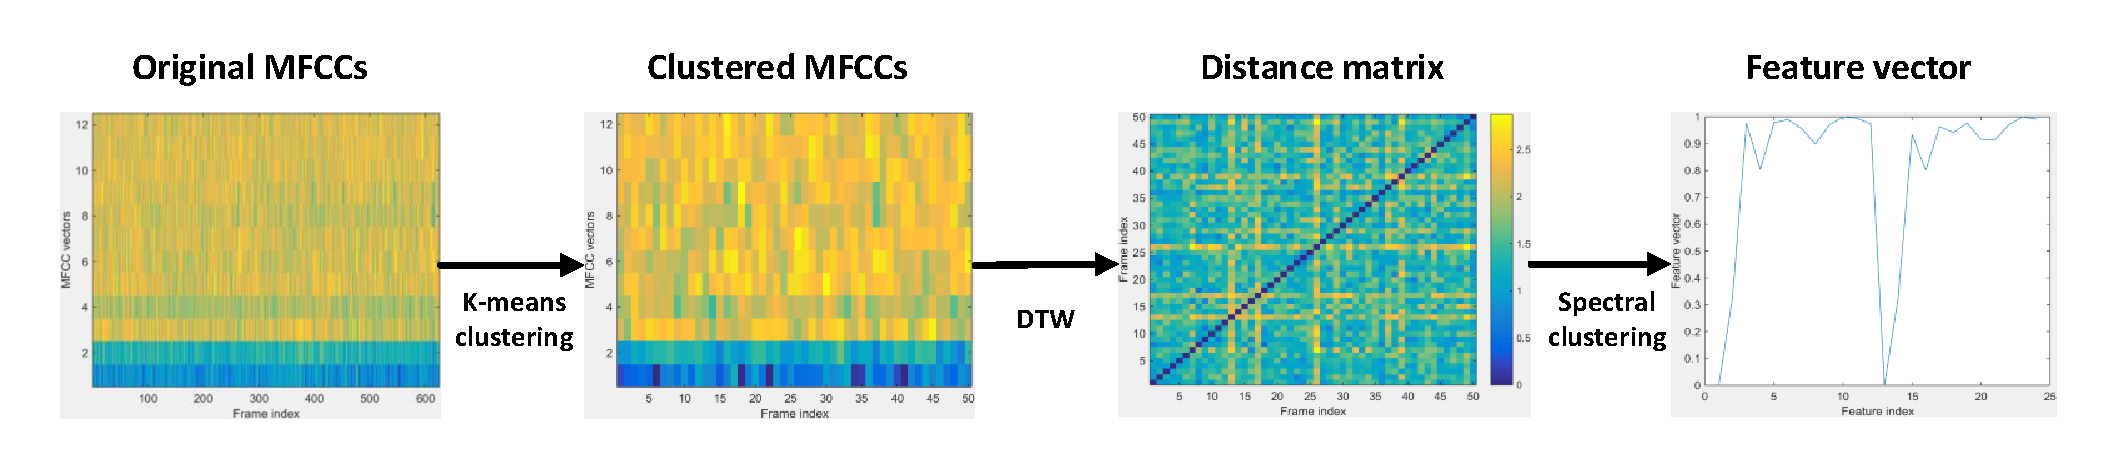
\includegraphics[width=\linewidth]{image/spectralClustering.pdf}}
\caption[Spectral clustering for cepstral feature extraction]{Procedure for extracting cepstral based feature vectors}
\label{fig:spectralClustering} 
\end{figure}





\subsection{Multi-label classification} 
Since many sampled recordings consist of calls from multiple frog species, frog call classification can be framed as a ML learning problem. However, previous studies have not adopted ML learning to classify frog calls. Therefore, it is worth investigating different ML learning algorithms for the classification of multiple vocalising frog species in field recordings for its scalability and flexibility \citep{read2011classifier}. The principle of the BR method is to solve a multi-label classification problem using multiple binary classifiers respectively. Similar to our previous work \citep{zhang2016using}, 
three classic single-label learning algorithms: decision tree, and multi-layer perceptron, and random forest. Here, random forest is selected as the base classifier, since our previous study of classifying frog species has already demonstrated its comparable performance \citep{xie2016acoustic}. 

\section{Experiment results}
Each 10-second recording is divided into frames of 512 samples and 50\% frame overlap for STFT. For MFCCs and AWSCCs, window size and overlap are 512 samples and 50\%, the window function is a Hamming window. All algorithms were programmed in Matlab 2014b except ML learning, which was implemented in Meka 1.7.7\footnote[4]{http://meka.sourceforge.net/}. 







\subsection{Evaluation metrics}
For multi-label classification, the performance evaluation differs from the classic single-label classification systems. The multi-label classification results often have a situation where partial labels are correctly predicted, but the prediction of single-label classification is either correct or incorrect. Therefore, some traditional evaluation metrics for the single-label classification, such as precision, recall, and accuracy, are no longer suitable for the multi-label classification system. In this study, three evaluation metrics, hamming loss, accuracy, and subset accuracy, are used, where all the three are example based measures \citep{madjarov2012extensive}.


The definition of Hamming loss can be found in Chapter~\ref{cha:cha6MIML}.
%Hamming loss is defined as the fraction of labels that are incorrectly predicted for an instance and the normalised hamming loss which is normalised over instances is reported. This metric is defined as
%\begin{equation}
%hammingLoss = \frac{1}{N}\sum_{i=1}^{N}\frac{1}{Q}|h(x_{i})\Delta y_{i})|
%\end{equation}
%where $\Delta$ denotes the symmetric difference between two instances,  and $Q$ is the total number of possible labels. 

Accuracy for a single instance $x_{i}$ is defined by the Jaccard similarity coefficients between the ground truth $y_{i}$ and the prediction $h(x_{i})$. Accuracy is micro-averaged across all examples:

\begin{equation}
accuracy = \frac{1}{N}\sum_{i=1}^{N}|\frac{h(x_{i} \cap y_{i})}{h(x_{i} \cup y_{i}}|
\end{equation}
where $N$ is the number of instances, $y_{i}$ denotes the ground truth of instance $x_{i}$, and $h(x_{i})$ denotes the predictions for the same instance. 


Subset accuracy is defined as follows:
\begin{equation}
subsetAccuracy = \frac{1}{N}\sum_{i=1}^{N}I(h(x_{i})=y_{i})
\end{equation}
where $I(true)=1$ and $I(false)=0$. This is a very strict evaluation
measure as it requires the predicted set of labels to be an exact
match of the true set of labels.


The values for hamming loss, accuracy, and subset accuracy range from 0 to 1. For hamming loss, 0 denotes the perfect result, and 1 means the wrong prediction of all labels over every instance, whereas for accuracy and subset accuracy, the values have the completely opposite meanings.



\subsection{Classification results}

Experiment results are shown in Table~\ref{tab:classificationResults}. The combination of LPCs, MFCCs, and AWSCCs, can achieve the best performance with ML-random forest. Using only cepstral coefficients, the best classification performance is achieve by AWSCCs(2), of which the accuracy is 0.662. After adding the temporal feature (LPCs), the accuracy is improved to 0.694. The reason for this improvement might be that this combination can achieve both temporal and frequency information of the recording. Compared to other classifiers, the classification performance of ML-RF is better than both ML-kNN and ML-DT (Table~\ref{tab:MLclassifierComparision}).



\begin{table}[htb!]
\centering
\caption{Comparison of different feature sets for ML classification. Here, MFCCs-1 and MFCCs-2 denote cepstral features are calculated via first and second methods, respectively}
\label{tab:classificationResults}
\resizebox{\textwidth}{!}{
\begin{tabular}{lllll}
\hline\hline
Feature set           & Base Classifier                             & Hamming loss $\downarrow$ & Accuracy $\uparrow$   & Subset accuracy $\uparrow$ \\ \hline
MFCCs-1                 & \multirow{5}{*}{Random forest} & 0.143 $\pm$ 0.015  & 0.64 $\pm$ 0.035 & 0.354 $\pm$ 0.052     \\ \cline{1-1} \cline{3-5} 
MFCCs-2                &            & 0.139 $\pm$ 0.01  & 0.659 $\pm$ 0.019 & 0.362 $\pm$ 0.036     \\ \cline{1-1} \cline{3-5} 
AWSCCs-1        &                                        & 0.139 $\pm$ 0.011  & 0.656 $\pm$ 0.009 & 0.371 $\pm$ 0.038     \\ \cline{1-1} \cline{3-5} 
AWSCCs-2 &                                        & 0.138 $\pm$ 0.012  & 0.662 $\pm$ 0.01 & 0.38 $\pm$ 0.031     \\ \cline{1-1} \cline{3-5} 
AWSCCs-2 + LPCs &                                        & \textbf{0.117 $\pm$ 0.011}  & \textbf{0.694 $\pm$ 0.027} & \textbf{0.424 $\pm$ 0.027}     \\ \hline\hline
\end{tabular}
}
\end{table}




\begin{table}[htb!]
\centering
\caption{Comparison of different ML classifiers}
\label{tab:MLclassifierComparision}
\resizebox{\textwidth}{!}{
\begin{tabular}{lllll}
\hline\hline
Feature set           & Base classifier            & Hamming loss $\downarrow$  & Accuracy $\uparrow$     & Subset accuracy $\uparrow$ \\ \hline
AWSCCs-2 + LPCs & ML-kNN                   & 0.139 $\pm$ 0.023  & 0.679 $\pm$ 0.039 & 0.362 $\pm$ 0.065     \\ 
AWSCCs-2 + LPCs & ML-Decision Tree         & 0.171 $\pm$ 0.012  & 0.593 $\pm$ 0.018 & 0.272 $\pm$ 0.036     \\ 
AWSCCs-2 + LPCs & ML-Random forest & 0.117 $\pm$ 0.011  & 0.694 $\pm$ 0.027 & 0.424 $\pm$ 0.027     \\ \hline\hline
\end{tabular}
}
\end{table}




\subsection{Comparison with MIML}
In this chapter, ML learning is used to classify frog calls without syllable segmentation. Compared to the MIML learning (Figure~\ref{fig:classificationResults} in Chapter~\ref{cha:cha6MIML}), the ML classification has a slightly better classification performance. For ML classification, LPCs, MFCCs, and AWSCCs are combined for the classification. MFCCs and AWSCCs are calculated by averaging cepstral features in the temporal direction. Although this process will compress the information in the temporal direction, the information of the cepstral domain is obtained. Since most frog species tend to continuously make calls, the compression of the temporal information will not greatly affect the discriminability of the ceptral features.
LPCs are added to get the temporal information. In contrast, features used for MIML classification are calculated from each segmented syllable. However, current AED often cannot accurately segment frog calls with low energies, which greatly affects the classification performance.


\section{Summary}
In this chapter, ML learning is used to classify multiple simultaneously vocalising frog species in field recordings. A combination of AWSCCs-1 and LPCs can achieve the best classification performance, which is similar with MIML classification results reported in Chapter~\ref{cha:cha6MIML}. To construct the final feature set, a novel method is proposed based on spectral clustering. Although the classification performance is similar with the statistical method, the feature dimension is greatly decreased from 72 to 24. Compared to MIML learning, ML learning does not need to segment frog syllables, which can increase the robustness of the classification results. Compared to other classifiers, ML-random forest can achieve the best classification performance with a hamming loss of 0.117. 





